%
% Beispiel mit der Klasse scrartcl
%

\documentclass[pdftex,a4paper,12pt]{scrartcl}
%\usepackage[ngerman]{babel}
\usepackage[utf8]{inputenc}
%\usepackage[T1]{fontenc}
% F�r die Schriftart times zu verwenden
%\usepackage{mathptmx}
%\usepackage[scaled=.90]{helvet}
\usepackage{courier}

\usepackage{longtable}
\usepackage{tikz}
\usepackage[siunitx,europeanresistors]{circuitikz}
\usepackage{pgfplots}
\usepackage{mathtools}
\usepackage{amsmath}
\usepackage{nicefrac}
\usepackage{booktabs}
\usepackage{float}
\usepackage{graphicx}
\usepackage{hyperref}
\usepackage{setspace}

\setlength{\parindent}{0em}
\onehalfspacing

%\usepackage{ragged2e}

\newcommand{\km}{\rule[0.6ex]{4pt}{0.8pt}} % kleineres Minus

\newcommand{\fb}[1] {
\framebox[1.2cm]{#1}}
%\fb{#1}}
\newcommand{\fs}[1] {
\footnotesize{#1} }
\newcommand{\nice}[2] {
\nicefrac{#1}{#2} }
\newcommand{\tb}[1] {
\textbf{#1} }

\title{A RPN Calculator for real and complex numbers}
\author{Andreas Thadewald}
\date{\today}

\begin{document}

\maketitle

\begin{abstract}
\textbf{Calculation of AC-Circuits and more!}\\
\begin{minipage}{0.2\textwidth}
\begin{figure}[H]
\centering
\begin{circuitikz}
      \draw (0,2)
      to[L=$L_{1}$, o-] (2,2) % The coil
      to[C=$C_{1}$, *-] (2,0) % The capacitor
      to[R=$R_{1}$, *-o] (0,0); % The resistor
      \draw (2,2)
      to[short, *-] (4,2)
      to[R=$R_{2}$, *-] (4,0)
      to[short, *-] (2,0);
      \draw (4,2)
      to[short, *-] (6,2)
      to[C=$C_{2}$, *-] (6,0) % The capacitor
      to[R=$R_{4}$, *-] (4,0);
      \draw (6,2)
      to[R=$R_{3}$] (8,2) % The resistor
      to[L=$L_2$] (8,0)
      to[short] (6,0);
\end{circuitikz}
\end{figure}
\end{minipage}
\end{abstract}

\tableofcontents
\newpage
 

\section{The calculator}
 
\begin{figure}[H]
	\centering
	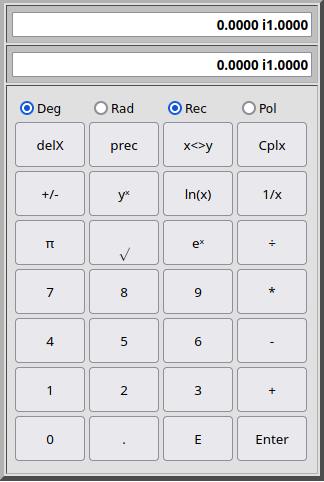
\includegraphics[scale=0.7]{Calculator.png} 
\end{figure} 
How to get the Values in the display like in the picture above: \\

1 \fb{Enter} 30  \fb{cplx} \fb{Enter} 1 \fb{$e^x$}
\subsection{Reverse Polish Notation (RPN)}
First the numbers, then the operator ($+$, $*$ ...). Example: 35 \fb{Enter} 14.7 \fb{$+$}.
\begin{table}[H] 
\centering
\begin{tabular}{|p{2cm}|p{3cm}|c|}
\hline
Field 	 & Stack 	&\\\hline
T		&	0.0000	&not visible\\\hline 
U		&	0.0000	&not visible\\\hline 
Y		&	0.0000	&visible\\\hline 
X		&	0.0000	&visible\\\hline 
\end{tabular} 
\end{table}
\begin{table}[H] 
%\centering
\begin{small}
\begin{tabular}{ccclclcclclc}
 
\multicolumn{12}{c}{Calculate \large{$\nice{(35 + 14.7) * 7}{(22.7 - 3.14)}$}} \\ 
		&			& 		&		 &			& 		 &	& 		  &		   &		&		&			\\
T		& 0.0000	& 		& 0.0000 & 			& 0.0000 &	& 		  & 0.0000 &		& 0.0000&		    \\
U		& 0.0000	& 		& 0.0000 & 			& 0.0000 & 	& 		  & 0.0000 &		& 0.0000&	        \\
Y		& 0.0000	& 		& 0.0000 & 			& 35.0000&	& 		  & 35.0000&		& 0.0000&	         \\
X		& 0.0000	&\tb{35}& 35     &\fb{Enter}& 35.0000&  &\tb{14.7}& 14.7	 &\fb{+}& 49.7000& \tb{7}
\end{tabular}
\end{small} 
\end{table}
\begin{table}[H] 
%\centering
\begin{small}
\begin{tabular}{clclclclcl}
T		& 0.0000	& 		& 0.0000 & 		   & 0.0000   &		  	 & 0.0000	&			\\
U		& 0.0000	& 		& 0.0000 & 		   & 0.0000   &		  	 & 347.9000	&			\\
Y		& 49.7000	& 		& 0.0000 & 		   & 347.9000 &		  	 & 22.7000	&			\\
X		& 7			&\fb{$*$} &347.9000&\tb{22.7} &22.7	  &\fb{Enter}& 22.7000 	&\tb{3.14}	
\end{tabular}
\end{small} 
\end{table}
\begin{table}[H] 
%\centering
\begin{small}
\begin{tabular}{clclcl}
T	& 0.0000		& 		& 0.0000 & 		   & 0.0000   \\
U	& 347.9000		& 		& 0.0000 & 		   & 0.0000   \\
Y	& 22.7000		& 		& 347.9000 & 	   & 0.0000 \\
X	& 3.14 			&\fb{$-$} &19.56&\fb{$/$}  & 17.7863	 
\end{tabular}
\end{small} 
\end{table}

\newpage{}

\section{Complex numbers}
Complex numbers are two-dimensional numbers, with a real- and imaginary part. Calculation is similar to binomial theorem.
\begin{align*}
(a+b)^2 &= a^2 + 2ab + b^2 \qquad \text{binomial theorem} \\
(a+ib)^2 &= a^2 + i2ab - b^2 = a^2 - b^2 + i2ab \qquad \text{Complex number}
\end{align*}
Get $-b^2$ because of $i^{2} = -1$.\\

There are two ways to represent complex numbers:
\begin{itemize}
	\item Rectangular coordinates (a + ib) \qquad (Rect)
	\item Polar coordinates $|r|*e^{i\varphi}$ mit $|r| = \sqrt{a^2 + b^2}$ \qquad (Pol)
\end{itemize}

%\subsection{Die komplexe Zahlenebene}
%% Beschreibung der komplexen Zahlenebene
%\newpage
\begin{figure}[H]
  \centering
\begin{tikzpicture}[
  font=\footnotesize, % kleinere Schrift
  samples=2, % zum Plotten von Geraden reichen 2 Punkte
  scale = 1.3
  ]
% Koordinatensystem
  \draw[-stealth](-3,0)--(3.2,0)node[below right,xshift=-3mm]{Re$(z)=a$};
  \draw[-stealth](0,-3)--(0,3)node[left]{Im$(z)=ib$};
  \clip(-3,-3)rectangle(3.2,3);
  \foreach \i in {1,2}\draw[very thin]
    (\i,2pt)--(\i,-2pt)node[below]{\i}
    (-\i,2pt)--(-\i,-2pt)node[below]{-\i}
    (2pt,\i)--(-2pt,\i)node[left]{\i}
    (2pt,-\i)--(-2pt,-\i)node[left]{-\i} ;
% polar coordinate
\draw (0,0)--(2,2)node[anchor=south west]{$\underline z = 2+i2$};
\draw [thin,dashed] (2,2)--(2,0);
\draw (0.5,1)node[anchor=west,rotate=45]{$|r|$};
\draw [fill=gray!30](0,0) -- (0.75,0) arc (0:45:0.75cm);
\draw (1,0.3) node[rotate=10]{$\varphi$};
\fill [black](2,2) circle(2pt);
%\draw (0,0)--(2,-2)node[anchor=north west]{$\underline z^{*}=2-2i$};
\draw [thin,dashed] (2,2)--(2,0);
\draw (0.5,1)node[anchor=west,rotate=45]{$|r|$};
%\draw [fill=green](0,0) -- (0.75,0) arc (0:-45:0.75cm);
%\draw (0.8,-0.3) node[rotate=10]{$-\varphi$};
%\fill [black](2,-2) circle(2pt);

\end{tikzpicture}
  \caption{complex number plane}
  \label{fig:complex number plane}
\end{figure}
\newpage
\section{Operating instructions}
The complex number 3 + i5 in rectangular coordinates (Rect):\\

\qquad 3 \fb{Enter} 5 \fb{cplx} \\

The real part 3 in the Y-Field and the imaginary part 5 in the X-Field.

\subsection{Trigonometric Functions}
Take a look at the complex plane, you see a right triangle with these relation
with the radius $r = 1$ of a circle.
\begin{align*}
&\cos^2a + \sin^2b = 1 \\
&\text{'Formular of Euler':} \\
&e^{i \cdot \varphi ^\circ} =  \cos(\varphi ^\circ) + i \sin(\varphi ^\circ))
\end{align*}
Calculation of sine, cosine and tangent of $\varphi = 30 ^\circ$ (Pol and Deg):\\

\qquad 1 \fb{Enter} 30 \fb{cplx} to Rect\\

because of the "Formular of Euler".\\ 
The input (Pol and Deg):

\begin{table}[H] \centering
\begin{tabular}{p{2cm}p{3cm}p{2cm}}

\toprule

Input	 			& X-Field					& Y-Field				\\
															
\midrule
1					& $1$						& 0.0000				\\
Enter				& $1.0000$ 					& $1.0000$				\\
30					& $30$  					& $1.0000$				\\
cplx				& 1.0000\: \angle 30.0000  	& 0.0000				\\
Rect				& $0.8660\: i0.5000 $ 		& 0.0000				\\
cplx				& $0.5000$  				& $0.8660$				\\
x$\Leftrightarrow$y	& $0.8660$  				& $0.5000$				\\
/					& $0.5774$  				& 0.0000 				\\

\bottomrule
\end{tabular} 
\end{table}

\vspace{0.5cm}

The $\sin(30 ^\circ) = 0.5$, the $\cos(30 ^\circ) = 0.866$.
The last value in the table is $\tan(30 ^\circ) = 0.5774$.\\
and backwards the atan (Rect and Deg):\\

\begin{table}[H] \centering
\begin{tabular}{p{2cm}p{3cm}p{2cm}}

\toprule

Input	 			& X-Field					& Y-Field				\\
															
\midrule
1					& $1$						& 0.5774				\\
x$\Leftrightarrow$y	& $0.5774$ 					& $1.0000$				\\
cplx				& 1.0000\: i0.5774  		& 0.0000				\\
Pol					& $1.1547\:\angle 30.0000 $ & 0.0000				\\

\bottomrule
\end{tabular} 
\end{table}

\subsection{Homers last theorem}
Calculation with big numbers. The Simpsons and 	Fermat's last theorem!
 
\begin{align*}
3987^{12} + 4365^{12} = 4472^{12}
\end{align*}
One of the author of the of the TV-series wrote a C-Programm to find this equation.
\begin{table}[H] \centering
\begin{tabular}{p{2cm}p{3cm}p{3cm}p{2cm}}
\toprule

Input	 			& X-Field					& Y-Field				&  U-Register    \\
															
\midrule
3987				& 3987						& 0.0000				&			   \\
Enter				& 3987.0000					& 3987.0000				&			   \\
12					& 12  						& 3987.0000				&			   \\
$y^x$				& 1.6134e+43				& 0.0000				&			   \\
4365				& 4365						& 1.6134e+43			&			   \\
Enter				& 4365.0000	  				& 4365.0000				& 1.6134e+43	\\
12					& 12  						& 4365.0000				& 1.6134e+43	\\
$y^x$				& 4.7842e+43				& 1.6134e+43			&			   \\
+					& 6.3977e+43				& 0.0000 				&			   \\
4472				& 4472						& 6.3977e+43			&			   \\
Enter				& 4472.0000	  				& 4472.0000				& 6.3977e+43	\\
12					& 12  						& 4472.0000				& 6.3977e+43	\\
$y^x$				& 6.3977e+43				& 6.3977e+43			&			   \\

\bottomrule

\end{tabular} 
\end{table}
The left and the right side of the equation are equal!. But the \fb{prec} toggle-button shows, that Fermat's last theorem
was not disproved.
\newpage

\section{Calculation of AC-Circuits}

\subsection{Simple Resistor-Circuit}
Calculation of $R_{total}$
\begin{figure}[H] % placed ?HERE? \usepackage{float}
\centering
\begin{circuitikz}
\draw   (0,0)  node[anchor=east] {} to[short, o-] (1,0)
		to[R=2<\ohm>, -*] 	(3,0) 
		to[R=3<\ohm>, *-*] 	(5,0) 
		to[R=1<\ohm>, *-] 		(7,0)
%   
        (3,0)  to[R=5<\ohm>, *-*]  (3,-2) 
         
        (5,0)  to[R=7<\ohm>, *-*]  (5,-2) 
%
        (7,0)  to[R=4<\ohm>,  -]  (7,-2) 
        
		(0,-2)  node[anchor=east] {} to[short, o-] (7,-2)
		(-0.3,-1)  node[anchor=east] {$R_{total}$ $\Rightarrow$} to[] (-0.3,-1);
				  
\end{circuitikz}
\caption{Resistor-Network}
\end{figure}
\footnotesize
\begin{align*}
R_{total} &= 2 \Omega + \cfrac{1}{\cfrac{1}{5 \Omega} + \cfrac{1}{3 \Omega + 
			\cfrac{1}{\cfrac{1}{7 \Omega} +
          	\cfrac{1}{1 \Omega + 4 \Omega}}}} 
\end{align*}
\normalsize
\begin{table}[H] 
\centering
\begin{tabular}{@{}p{2.5cm}p{3cm}p{2cm}@{}}
\toprule
Input	 			& X-Field				& Y-Field			    \\
\midrule
1					& $1$					& 0.0000				\\
Enter				& $1.000$ 				& $1.0000$				\\
4					& $4$  					& $1.0000$				\\
+					& $5.0000$  			& 0.0000				\\
\nicefrac{1}{x}		& $0.2000$  			& 0.0000				\\
7					& $7.0000$				& $0.2000$  			\\
\nicefrac{1}{x}		& $0.14286$  			& $0.2000$ 				\\
+					& $0.34286$				& 0.0000				\\
\nicefrac{1}{x}		& $2.91667$  			& 0.0000  				\\
3					& $3$  					& $2.9167$				\\
+					& $5.9167$				& 0.0000				\\
\nicefrac{1}{x}		& $0.1690$  			& 0.0000  				\\
5					& $5$  					& $0.1690$				\\
\nicefrac{1}{x}		& $0.2000$  			& $0.1690$				\\
+					& $0.3690$				& 0.0000 				\\
\nicefrac{1}{x}		& $2.7099$  			& 0.0000  				\\
2					& $2$  					& $2.7099$ 				\\
+					& $4.7099$				& 0.0000				\\

\bottomrule
\end{tabular}
\normalsize
\end{table}

\subsection{Circuit with complex resistors}

Calculate $Z_{total}$ and the current ${I}$ (Select Rect and Deg).

\begin{minipage}{0.3\textwidth}
 ${U}$ = 5V \\
 ${Z_1} = 200\Omega + i100\Omega$ \\ 
 ${Z_2} = 100\Omega - i50\Omega$ \\ 
 ${Z_3} = 150\Omega + i150\Omega$ \\ 
\end{minipage}
\begin{minipage}{0.3\textwidth}
\begin{figure}[H]
\centering
\begin{circuitikz}
      \draw (0,0)
	  to[sinusoidal voltage source=${U}$, -] (0,2)
	  to[R=${Z_1}$,i>^=${I}$, -*]   ( 4,2);
      \draw (4,2)
	  to[R=${Z_2}$, -]  (4,0);
      \draw (4,2)
      to[short] (6,2)
	  to[R=${Z_3}$, -]  (6,0)	  
      to[short, -] (4,0)
      to[short, *-] (0,0);
\end{circuitikz}
\end{figure}
\end{minipage} 
\vspace{1cm}

${Z_{total}} = {Z_1} + \dfrac{1}{\dfrac{1}{{Z_2}}+\dfrac{1}{{Z_3}}}$ and \quad
${I} = \dfrac{{U}}{{Z_{total}}}$ \\
\begin{table}[H] \centering
\begin{longtable}{p{2cm}p{4cm}p{4cm}p{4cm}}

\toprule
Input	 			& X-Field				& Y-Field				&  U-Register   \\
															
\midrule
\endhead
100					& $100$					& 0.0000				&					    \\
Enter				& $100.0000$ 			& $100.0000$			&					   \\
50					& $50$  				& $100.0000$			&					    \\
\nicefrac{+}{-}		& $\km50$  				& $100.0000$			&					    \\
cplx				& $100 \: i\km50$		& 0.0000				&					    \\
\nicefrac{1}{x}		& $0.0080\: i0.0040$  	& 0.0000  				&					    \\
150					& $150$  				& $0.0080\:i0.0040$ 	&					   \\
Enter				& $150.0000$ 			& $150.0000$			& $0.0080\:i0.0040$ 	   \\
cplx				& $150.0000\: i150.0000$& $0.008\: i0.004$		&					    \\
\nicefrac{1}{x}		& $0.0033\:i\:\km0.0033$&  $0.008\: i0.004$		&					   \\
+					& $0.00113\:i0.0007$	& 0.0000				&					   \\
\nicefrac{1}{x}		& $87.9310\:i\:\km5.1724$ & 0.0000  			&					    \\
200					& $200$  				& $87.9310\:i\:\km5.1724$ 		&					   \\
Enter				& $200.0000$ 			& $200.0000$			& $87.9310\:i\:\km5.1724$ 	   \\
100					& $100$ 				& $200.0000$			& $87.9310\:i\:\km5.1724$ 	   \\
cplx				& $200\: i100$			& $87.9310\:i\:\km5.1724$	&					    \\
+					& $287.9310\:i94.8276$	& 0.0000				&				    \\
5					& $5$  					& $287.9310\:i94.8276$	&			  \\
x$\Leftrightarrow$y	& $287.9310\:i94.8276$ & $5.0000$				&				    \\
/					& $0.0157\:i\:\km0.0052$& 0.0000  				&				    \\
Pol					& $0.0165\: \angle \km18.2288$	& 0.0000		&				    \\

\bottomrule
\end{longtable}
\end{table} 
\begin{align*}
{Z_{total}} = 287.9310 \Omega + i 94.8276 \Omega & \quad \text{and} \quad{I} = 16.5 mA * e^{\km18.2288} &
\end{align*} 

\newpage{}

\subsection{Circuit with coils and capacitors}

Calculate $Z_{total}$ (Select Rect and Deg).

\begin{minipage}{0.5\textwidth}
 $\omega = 100 Hz$ \\
 $L1 = 0.5H$, $L2 = 1H$ \\
 $C1 = 500\mu F$, $C2 = 100\mu F$ \\
 $R1 = 20\Omega$, $R2 = 50\Omega$, $R3 = 50\Omega$, $R4 = 30\Omega$
\end{minipage}
\begin{minipage}{0.2\textwidth}
\begin{figure}[H]
\centering
\begin{circuitikz}
      \draw (0,2)
      to[L=$L_{1}$, o-] (2,2) % The coil
      to[C=$C_{1}$, *-] (2,0) % The capacitor
      to[R=$R_{1}$, *-o] (0,0); % The resistor
      \draw (2,2)
      to[short, *-] (4,2)
      to[R=$R_{2}$, *-] (4,0)
      to[short, *-] (2,0);
      \draw (4,2)
      to[short, *-] (6,2)
      to[C=$C_{2}$, *-] (6,0) % The capacitor
      to[R=$R_{4}$, *-] (4,0);
      \draw (6,2)
      to[R=$R_{3}$] (8,2) % The resistor
      to[L=$L_2$] (8,0)
      to[short] (6,0);
\end{circuitikz}
\end{figure}
\end{minipage}
\vspace{1cm}

$Z_{1} = X_{C_{2}} || (X_{L_{2}} + R_{3}): 200\: i\:\km100$ \\
$Z_{2} = [(Z_{1} + R_{4}) || R_{2}] || X_{C_{1}}: 7.3442 \: i\:\km16.0160$ \\
$Z_{total} = Z_{2} + R_{1} + X_{L_{2}} : 27.3442 \: i33.9840$ \\

The input in the calculator: \\

\begin{itemize}
	\item \hspace{1cm} 100 \fb{Enter} 100E6 \nice{+}{-} $*$ \fb{cplx} 
	\item \hspace{1cm} 0  \fb{Enter} 100 \fb{cplx} 50 $+$ \nice{1}{x} $+$ \nice{1}{x}
	\item \hspace{1cm} 30 $+$ \nice{1}{x} 50 \nice{1}{x} $+$ 0  \fb{Enter} 100 \fb{Enter} 500E6 \nice{+}{-} $*$ \fb{cplx} $+$ \nice{1}{x}
	\item \hspace{1cm} 20 $+$ 0 \fb{Enter} 100 \fb{Enter} 0.5 $*$ \fb{cplx} $+$ 
\end{itemize}

\end{document}

%
% EOF
%


